\subsection{Study area: Lisbon, Portugal}
Lisbon is the capital city of Portugal, located close in the central west area of the continental country, just North of the River Tejo. Half a million people reside within the municipality of Lisbon, a total of 2.9 million in the Área Metropolitano de Lisboa (a Nomenclature of Territorial Units for Statistics NUTS II region \cite{eurostat} of 17 municipalities both north and south of the River Tejo), and 2.3 million in the overlapping Distrito de Lisboa (16 municipalities, entirely North of the river) \cite{censos2021}.

{\color{red}IMAGE OF DISTRICT VS AML VS MUNICIPIO}

Within the lisbon area, a variety of organizations serve communication media to the population, including such commercial endeavors as Público, Diário de Notícias, Jornal de Notícias, Observador, and at least ten other major news sources. Many of these have at least partially transitioned to an online presence, with some availabe exlusively online. A Mensagem, for example, is a newer addition to the news scene in Lisbon, is available exclusively online with some stories in the audio podcast format. This particular source is specifically aimed at hyperlocal information for the Lisbon community. Additionally, the Câmara Municipal de Lisboa solicits regular boletins and notícias, as do many of the juntas de freguesias within the municipality and beyond. News is heavily embedded in the culture, with many cafes and restaurants often streaming news channels and printed media available at kiosks at corners throughout the area. There is also a history of pirate radio in Portugal which contributed to the decentralization of speech\cite{Bonixe2019}. %-Independent Radio {“The end of the 70s marked the appearance of several pirate radios in Portugal beginning a process that would lead to the liberalization of the radio sector at the end of the following decade. For eleven years, several hundred small radios have broad-casted without a license bringing the voices of local people.”\cite{Bonixe2019}}; {“Os principais impulsionadores do fenómeno da radiodifusão local portuguesa referiam frequentemente a importância da existência de um discurso descentralizado e da partilha do processo de decisão sobre a coisa pública.” The main catalysts of the local portuguese pirate radios frequently refer to the importance of the existence of decentralized speech and the sharing of the public decision making process.\cite{Bonixe2019}};
Portugal more generally also has taken an interest in innovative journalism; João Palmeiro, president fo the Portuguese Publishers Association, chairs Google's Digital News Innovation Fund (DNI Fund), for quality journalism in Europe, which both supports portuguese media projects and includes commercial and academic Portuguese partners \cite{DNIFund2018}. %  DNI Fund {\color{orange}Portugal has taken an interest in innovative journalism: João Palmeiro (president of the Portuguese Publishers Association) chairs the DNI Fund, which both supports portuguese projects (Alberto Pereira, Cofina Media, Empresa jornalistica, região de leiria, global notícias, global notícias publicações, impresa, impresa publishing, INESC TEC, João Antunes, Agência de Notícias de Portugal [LUSA]) and includes Portuguese partners (Platforma de media privados, Público, Público: communicação social, Ricardo Lafuente, Universiety of Porto, and Visapress). \cite{DNIFund2018}}\\
%\subsubsection{Local news serving Lisbon}
%\begin{itemize}
%	\item Commercial media
%	\begin{itemize}
%		\item Público
%		\item Diário de Notícias
%		\item Jornal de Notícias
%		\item Correio da Manhã
%		\item Lisboa Euronews
%		\item Exame
%		\item Jornal Finanças
%		\item Expresso
%		\item Agência Lusa
%		\item TSF
%		\item Destak
%		\item Sapo
%		\item Notícias ao Minuto
%		\item Observador
%		\item Jornal I
%	\end{itemize}
%	\item Public media
%	\begin{itemize}
%		\item Boletim Municipal Câmara de Lisboa
%		\item CML Notícias
%		\item Juntas de Freguesia: notícias, newsletters, agendas, etc.
%	\end{itemize}
%	\item Independent
%	\begin{itemize}
%		\item {\color{red}identify}
%	\end{itemize}
%\end{itemize}

The hilly and water-lined layout of the city lends rich and distinct character to neighborhoods throughout the metropolitan area. Some of these cultures have persisted through decades, like the areas of Alfama and Alvalade, while others are constantly forging new identities and even rebranding themselves to invite new stories to be told, such as the Martim Moniz and Marvila areas. This, then, makes Lisbon an interesting case study to test a spatial news visualization, to see if the heterogenous personalities will be reflected in any geospatial patterns.




%\subsubsection{Views}
%The following views describe a variety of products that stem from the same geodatabase, though can be implemented indepenently and illustrate the initial opportunities of a such an online geospatial tool.
%\begin{enumerate}
%	\item A spatial database of incidents that supports the association of spatial, temporal, and thematic attributes. See Appendix \ref{appendix:organization}/Figure \ref{fig:data_model}: data model.
%	\item A POC Input tool for publishers that allows users to define the place(s) (drawing georeferrenced polygons on a map) as well as time of occurrence of incidents. It shall also, of course, preserve or potentially improve upon the association of traditional thematic attributes and keyword search. See Appendix \ref{appendix:organization}/Figure \ref{fig:input_ui}: \textit{Input} layout.
%	\item A POC Context map (visualization of an incident on a local map) for integration into each article page. See Appendix \ref{appendix:organization}/Figure \ref{fig:context_ui}: \textit{Context} layout.
%	\item A POC Search tool for researchers that allows users to filter by spatial (one or multiple defined places or via drawn definition of the study area), temporal, and or thematic attributes. The results should be displayable via both map and list views, as well as support CSV export functionality. See Appendix \ref{appendix:organization}/Figure \ref{fig:search_ui}: \textit{Search} layout.
%	\item A POC Dashboard tool for monitors (publisher, city officials, etc.) to monitor the spatial/temporal development of incidents according to their settings. 
%\end{enumerate}


	
%\subsection{Geo tools}

\subsection{Requirements}
%\textit{See Appendix \ref{appendix:organization}}\\
%-{\color{orange}Limit classification complexity. \cite{Jiang2020}}\\

The Apregoar system architecture reflects the needs of the browsers, researchers, monitors, and publishers anticipated to use the various functions of the tool, as per the earlier description and the following specifications:

\begin{itemize}
	\item{} The system should support all create read update and delete (CRUD) operations, though most views will only require reading of selected database records. This should include text, date, and spatial types.
	\item{} The system should be implemented with no or low cost maintenance.
	\item{} The system should support open source applictions, and therefore utilize openly licenced tools as much as possible.
	\item{} The system targets non-professional GIS users, and therefore should be straightforward and easy to use.
	\item{} The system will use spatial, thematic, and temporal filtering, and will therefore leverage dataframes that can support this type of rapid processing. Likewise, definition of such filters in an easily understood format are necessary.
	\item{} Users should be able to define polygons. This is applicable both in the georeferencing of incidents, which will therefore saved as a or multiple polygon type records, as well as for defining spatial search areas for use in filtering georeferenced articles.
	\item{} The main search results will be in map and list formats. Therefore, the system must support this type of data viewing.
	
\end{itemize}
\subsection{System architecture}
The Apregoar platform components were selected based on the above requirements, as well as the functionality described in the previous section. Also considered were the functionality of potential tool, available official and community resources, as well as prior experience in the options.

An event model requires spatiotemporal and attribute elements, with the former requriing specific formats and processing for data manipulation and storage. For this reason, the data storage leverages PostgreSQL with a Postgis extension for its vector data storage capabilities, support in literature (\cite{Oliveira2021,Bhattacharya2018,Teitler2008,Sami2019}), support for remote connection via python using related packages, and personal experience with the platform. 

%\subsection{GIS design}
%An event model requries spatiotemporal and attribute elements, with the former requiring specific formats and processing for data manipulation and storage.
%- Database: PostgreSQL \cite{Oliveira2021,Bhattacharya2018,Teitler2008,Sami2019}\\
%- PostGIS \cite{Bhattacharya2018, Sami2019}\\
%-{\color{orange}Geonode: open source platform for collaborating geo-spatial data; Geonode/GeoNetwork/Django/GeoExt: “provide a platform for sophisticated web browser spatial visualization and analysis”}\cite{Bhattacharya2018}\\

Connecting the database to the web application is an Apache server for its ease of implementation. For serving spatial features, Geoserver was selected for its vector data support, its documentation, support in literature (\cite{Bhattacharya2018,Jiang2020,Sami2019}) and prior experience. 
%\subsection{Web Interface}
%- API\cite{Jiang2020}\\
%- OGC WMS, CSW \cite{Bhattacharya2018,Jiang2020}\\
%- GeoServer \cite{Bhattacharya2018,Jiang2020,Sami2019}\\

%\subsection{Architecture}
%-{\color{purple}Choose dynamic hosting for an application driven site\cite{Low2020}}\\
%-{\color{purple}Drupal as content management system (CMS)\cite{Low2020}}\\
%-{\color{purple}Shared hosting is presumably sufficient: cheap, easy to manage, low traffic volume\cite{Low2020}}\\
%-{\color{purple} Confirm external database linking\cite{Low2020}}\\


The backend is based on a the Flask web development platform, chosen for its lightweight implementation and python programming language. Key libraries include Shapely, Geopandas, SQLalchemy, geoalchemy2, and Gdal.
%\subsection{Backend}
%- GeoExt \cite{Bhattacharya2018}\\
%- {\color{orange}“Open Geogrpahic Modeling System (Open GMS) provides specific data process services (including data mapping services, refactoring services, and visualization services) beyond traditional data services to help modeler to prepare suitable data for geographic simulation the open web environment.\cite{Jiang2020}}\\
%- OpenSearch: navigation of gazetteers \cite{Jiang2020}\\
%- Google address autocomplete \cite{Fitoussi}\\ %{\color{orange}“Drag the market to the location on a map, pick from suggested results using Google address autocomplete while typing an address, enter coordinates, or manually enter the address fields.”\cite{Fitoussi}}
%- Python \cite{Sami2019}\\
%\begin{itemize}
%	\item Shapely \cite{Sami2019}
%	\item Geopandas \cite{Sami2019}
%	\item Gdal \cite{Sami2019}
%	\item Pyproj \cite{Sami2019}
%\end{itemize}
%- Geodjango \cite{Sami2019}\\

For mapping visualization in the front, Open Layer and Map Box were both considered. Open Layers better adheres to open source standards, though to streamline the proof-of-concept development phase, MapBox was implemented due to its prior experience, as well as integration of a variety of functionality via its javascript library that supports many of the operational, yet not focal, functionality of this project.
%\subsection{Front end}
%- Leaflet \cite{Sami2019, Fitoussi}\\
%- Openlayers \cite{Bahattacharya2018, Sami2019}\\
%- GoogleMaps API \cite{Fitoussi}\\
%- OpenStreetMaps \cite{Fitoussi}\\
%\subsection{Manipulation}
%- Leaflet Boundary Canvas\\
%- Free draw\\
%- GeoAnnatator: {supports human annotators \cite{Karimzadeh2019}}

Any data preparation or local testing utilized QGIS, also for its adherence to open standards, prior experience, and literature support (\cite{Sami2019}).
%\subsection{Dataprep}
%- QGIS \cite{Sami2019}\\

\subsection{Relational data model}
The data relates potentially multiple spatial definitions to a particular news story via the association with instances, which layer back in the temporal element of each story. Users are also defined such that published articles can be edited by those who created those records, and then associated with activity of that user (or set of affiliated users, if applicable). This relationship is outlined in Figure \ref{fig:data_model}.

\begin{figure}[H]
	\centering
	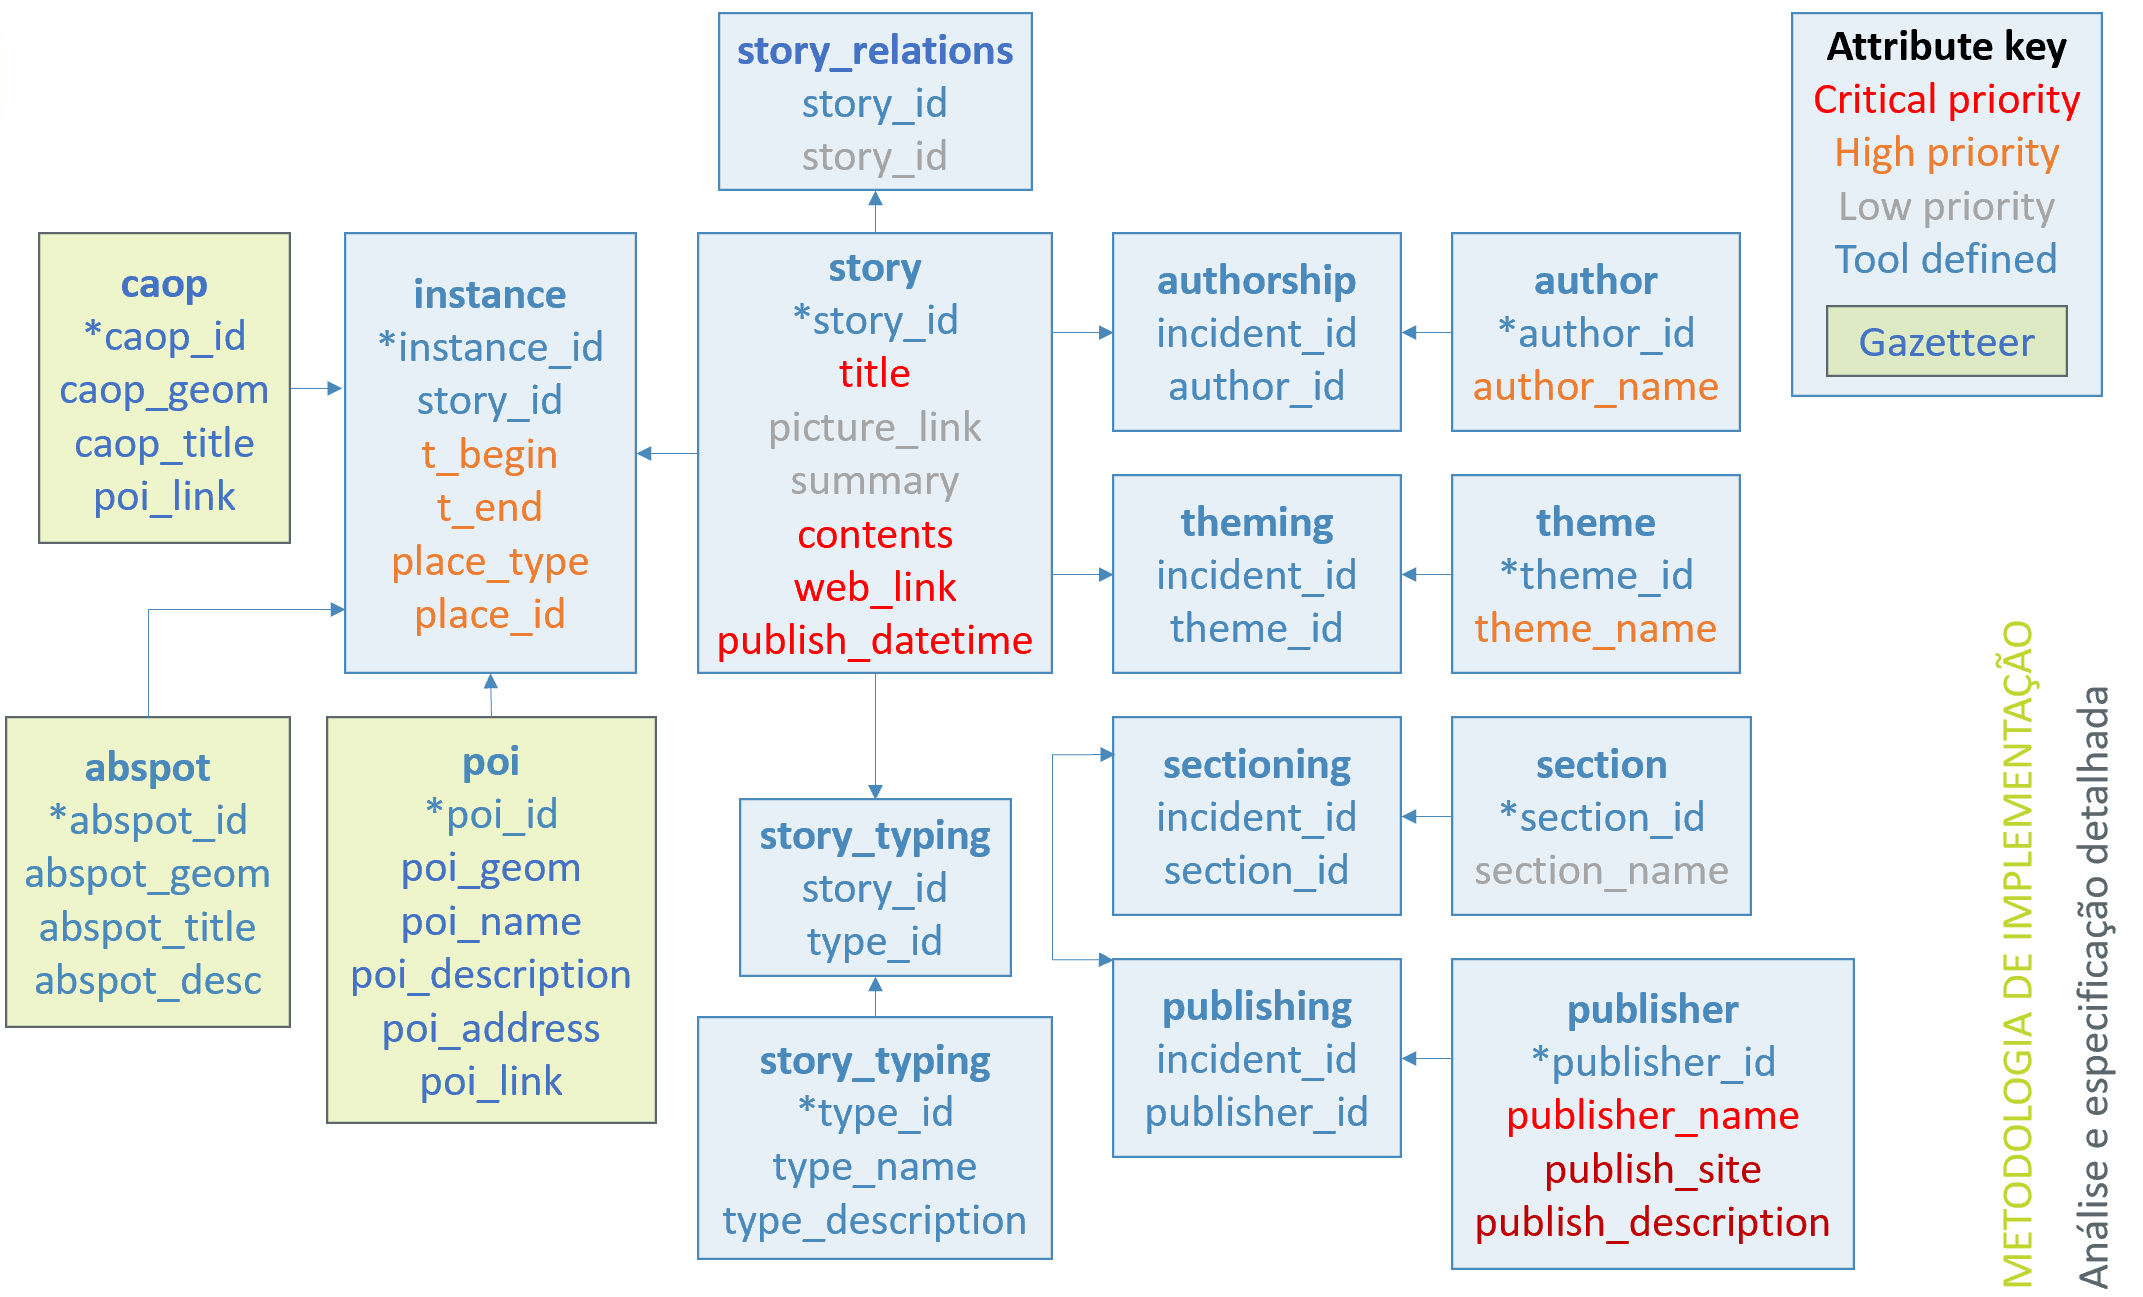
\includegraphics[width=.9\linewidth]{images/data_model.png}
	\caption{Data model}
	\label{fig:data_model}
\end{figure}

Publishers can associate spatiotemporal and thematic attributes to the stories they publish, reference to which is stored in a geodatabase. Only publishers perform any sort of data manipulation (create, update, delete) operations, while the remaining views simply read the data stored within. 

\subsection{Data Collection}
\subsubsection{Corpora}
The following corpora is selected as a representation of event reports for the month of October, 2020. It incorporates public organization (Municipality and selected Freguesias) as well as private newsmedia sources to inform the organiational rubric and data model.  

%-{\color{red} Use RSS feeds of publications as a source of data input\cite{Rivera2020}}\\

\begin{table} [H]
		\centering
		\begin{tabular}{| l l l l l |}
			\hline
			Source & Data & \# & Contents' dates & Scale \\ 
			\hline
			\hline
			CML & Boletim 1392 & 36 & Mar - Oct20 & address - municipality \\ 
			 & Notícias & 42 & {\color{red}Oct20}  & {\color{red}sub-bairro} \\ 
			 \hline
			JFC & Notícias & 21 & Sep - Dec20 & sub-bairo - freguesia \\
			& Newsletter & && \\
			\hline
			JCE & Agenda & 4 & Jun-Dec20 & freguesia \\
			 & Notícias & 10 & Oct20-Jan21& address - freguesia \\
			 \hline
			Público* & ípsilon & 83 & {\color{red}Oct20-2030} & {\color{red}address - inter-municipality} \\
			& impar  &  &  &  \\
			& Público  &  &  &  \\
			& Fugas &  &  &  \\
			& p3  &  &  &  \\
			& (uncategorized)  &  &  &  \\
%			Hyperlocal news & {\color{red}XX} & {\color{red}XX} & {\color{red}XX} & {\color{red}XX} \\
			\hline
			\hline
			\textbf{Total} & \textbf{} & \textbf{{\color{red}196}} & \textbf{{\color{red}Mar20-2030}} & \textbf{{\color{red}address - inter-municipality}} \\
			\hline
		\end{tabular}
		\caption{Corpora data}
		\label{table:data_corpora}
\end{table}

\textit{*Público data was procurred via the website's search feature, which includes results from all of their products.  The filters used were keyword ''LISBOA'' published during October 2020. }

All attributes are copied direclty from the source materials, with the exeption of times and places. These are extracted from the corpora, as these elements may not be explicitys stated (``yesterday'' or ``near the road'' or ``on his birthday''). Required fields indicate those that must be extractable from articles to be included in the corpora. Priority fields are ideally included, and efforts to extract this data will be made if not immediately obvious. If not applicable, these fields may remain blank. Other fields are helpful but not critical for inclusion.

\begin{table} [H]
		\centering
		\begin{tabular}{| l l l l p{5cm} |}
			\hline
			\textbf{Attribute} & \textbf{Type} & \textbf{Priority} & \textbf{Visibility} & \textbf{Note} \\
			\hline
			Title & Text & Critical & Yes & \\
			Summary & Text & Low & Maybe & Keyword search priority \\
			Contents & Text & High & No & Keyword search \\
			Photo & Web link & Low & Maybe & \\
			Section & Text & High & Yes & Thematic filtering \\
			Themes & Text & High & Yes & Thematic filtering \\
			Times & Text list & High & Yes & Temporal filtering \\
			Places & Text list & High & Yes & Geospatial filtering \\
			Referenced articles & Web link & Low & Maybe &Suggestion \\
			Related articles & Web link & low & Maybe &Suggestion \\
			Author & Text & High & Yes & \\
			Source & Text & Critical & Yes & \\
			Publication date & Date & Critical & Yes & Default temporal filtering and extraction\\
			Link & Web link & Critcal & Yes & \\
			\hline
		\end{tabular}
		\caption{Corpora attribute collection}
		\label{table:data_corpora}
\end{table}

\subsubsection{Basemaps}
\begin{table} [H]
		\centering
		\begin{tabular}{| l l l l l |}
			\hline
			Source & Name & \# Records & Geometry & SRS \\ 
			\hline
			\hline
			CML Geodados & Quarteirões & 1086 & Area & EPSG:4326 \\
			& Grandes parques e jardins de lisboa & 190 & Area & EPSG:4326 \\
			& Rede viária & 3763 & Line &  EPSG:4326 \\
			& Limite do conselho & 1 & Area & EPSG:4326 \\
			& Rede ferroviária subterrânea & 1 & Line & EPSG:4326 \\
			\hline
			DGTerritório & CAOP 2019 - Continental & 3,223 & Area & EPSG:3763 \\
			\hline
			& {\color{red}Bairros} &  &  &  \\
			\hline
			& {\color{red}Address} &  &  &  \\
			\hline
			\hline
			\textbf{Total} & & \textbf{ \textbf{\color{red}8,224}} & & \\
			\hline
		\end{tabular}
		\caption{Base map data}
		\label{table:data_basemaps}
\end{table}

\subsubsection{Gazetteers}
-{\color{red} Include feature codes from GeoNames to help with disambiguation of human annotators selecting toponyms\cite{Karimzadeh2019}}\\
\begin{table} [H]
		\centering
		\begin{tabular}{| l l l l l |}
			\hline
			Source & Name & \# Records & Geometry & SRS \\ 
			\hline
			\hline
			GeoNames & PT&37327 & Point & WGS84 \\
			\hline
			OSM PT & Waterways & 49,376 & Line & WGS84 \\
			&  & 54,041 & Area & WGS84 \\
			& Transport & 18,696 & Point & WGS84 \\
			& & 1,078 & Area & WGS84 \\
			& Traffic & 84,756 & Point & WGS84 \\
			&  & 35,339 & Area & WGS84 \\
			& Roads & 1,035,765 & Line & WGS84 \\
			& Railways & 8,310 & Line & WGS84 \\
			& POIs & 100,214 & Point & WGS84 \\
			&  & 71,335 & Area & WGS84 \\
			& POWs & 2,133 & Point & WGS84 \\
			&  & 7,358 & Area & WGS84 \\
			& Places & 23,594 & Point & WGS84 \\
			&  & 1,971 & Area & WGS84 \\
			& Natural & 89,483 & Point & WGS84 \\
			&  & 1,369 & Area & WGS84 \\
			& Landuse & 209,330 & Area & WGS84 \\
			& Buildings & 1,060,745 & Area & WGS84 \\
			\hline
			\hline
			\textbf{Total} & & \textbf{2,892,220} & & \\
			\hline
		\end{tabular}
		\caption{Gazetteer data}
		\label{table:data_gazetteer}
\end{table}

\begin{figure}[H]
	\centering
	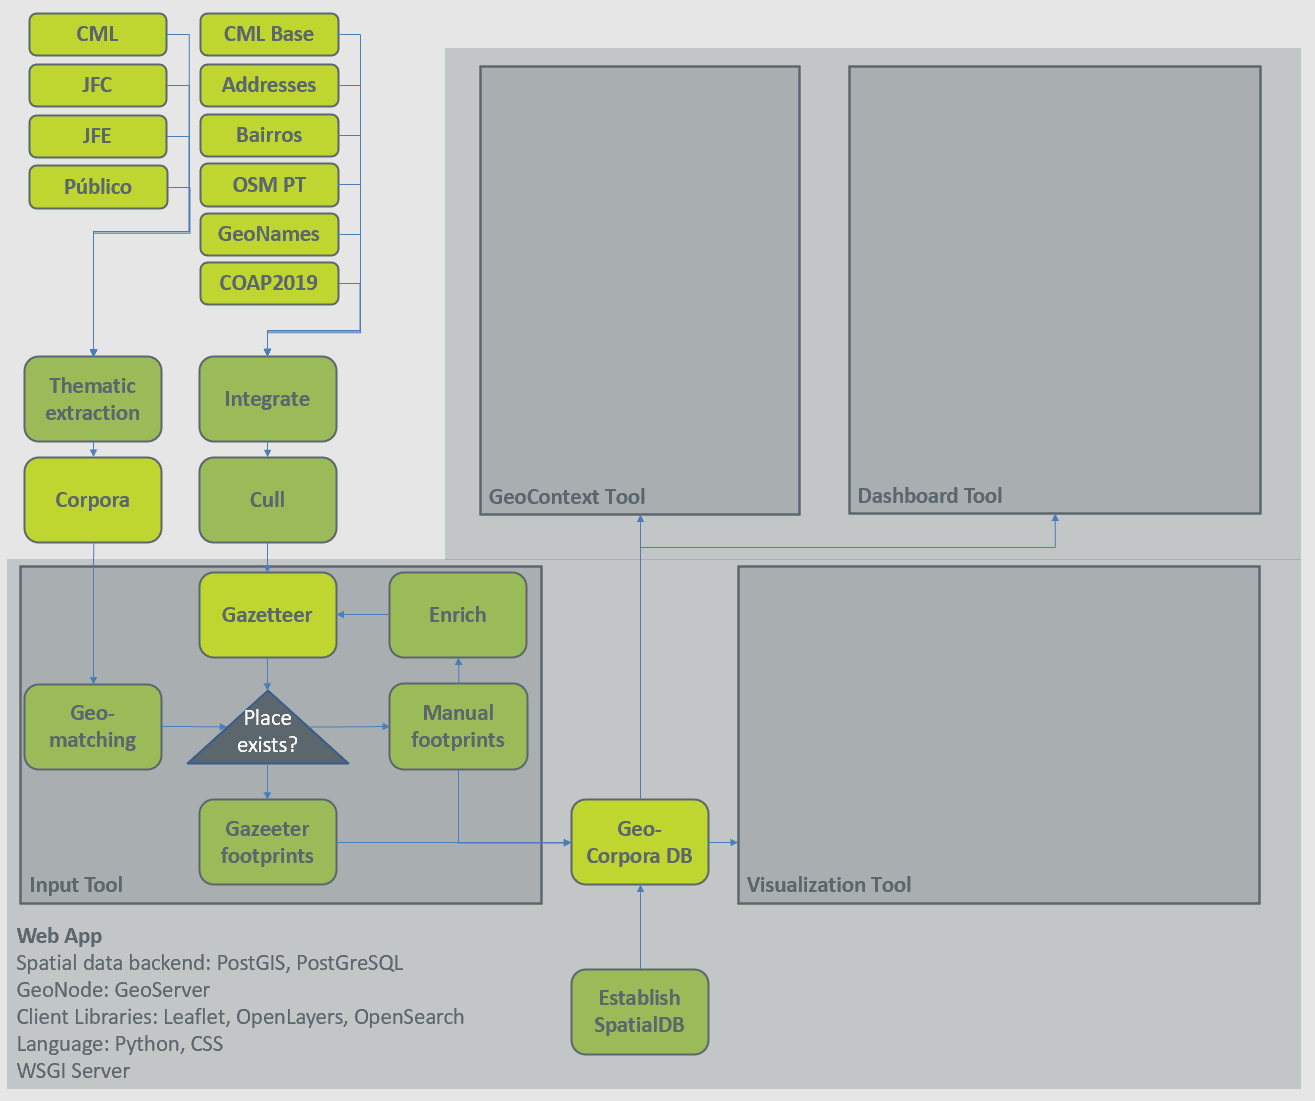
\includegraphics[width=.9\linewidth]{images/method_model.png}
	\caption{Preliminary methodology}
	\label{fig:method_model}
\end{figure}

\subsection{Preprocessing}
Load all gazetteer data into QGIS.
Establish georeference (note in data breakdown), transform as necessary
Manually code all article data. Using multiple sources to ensure continuity across local data sources.

\subsection{Initialization of development environment}
Selection and integration of resources and tools:
\begin{itemize}
	\item Database: PostgreSQL
\end{itemize}
Establish geodatabase structure, accommodating multiple language options, load gazetteer(s) and relevant administrative boundary data
Develop and test Input tool: wordpress plugin?
Develop and test search tool
Develop and test Context tool
Translate web app content to portuguese and load translations
Migrate site to the server
Test system
Compare results against mined location results
Document results

Future development: dashboard tool

\subsection{Tool design}
-{\color{red}Define design requirements and views to achieve them\cite{Zhang2019}}\\

\subsection{Testing}
- {\color{red}Test in different browsers for feature functionality.\cite{Shneiderman2020}}\\

\subsection{Validation}
1. GDELT: compare Lisbon Oct 2020 to results
2. Automatic extraction over sample corpora to compare results {\color{red} leverage Rivera2020 study}
- spaCy
-{\color{orange}``Large scale infomration extraction tasks''\cite{spaCy2020}}\\
-{\color{orange} Free online classes to learn\cite{spaCy2020}}\\
-{\color{purple}Utilize NER to extract exact and complete places.  As a baseline comparison to the input tool? Used together? Feed through the system with a “check point” (verify the identified place before input)?\cite{Gupta2020}}\\
-{\color{red}Use local datasets (Público, CML, Freguesia) from 1 month of each to build and test a backoffice plugin for defining localization of news articles. Ask MAGG or similar to apply the plug in for upcoming articles for a 1 month period and test against the same dataset with NewsStand. Is it richer/more accurate? Is the journalist satisfied with the result? Is the reader? Load the same local base gazetteer (OSM Portugal and Global)\cite{Lieberman2010}}\\
-{\color{red}Use method for extraction on input articles to extract and geolocate place for input comparison to automated methods?? Python and Restful API}\\
